\documentclass[12pt]{article}
\usepackage[margin=1.0in]{geometry}
\usepackage{amsmath}
\usepackage{amsthm}
\usepackage{amsfonts}
\usepackage{amssymb}
\usepackage{latexsym}
\usepackage{graphicx}
\usepackage{listings}
\usepackage{titling}
\usepackage{setspace}
\usepackage[utf8]{inputenc}
\usepackage[english]{babel}
\usepackage{hyperref}
\usepackage{algpseudocode}

\usepackage{xcolor}
\usepackage{listings}
\setcounter{secnumdepth}{4}
\lstset{
    frame=single,
    breaklines=true,
    postbreak=\raisebox{0ex}[0ex][0ex]{\ensuremath{\color{red}\hookrightarrow\space}}
}

\newtheorem{definition}{Definition}[section]
\newtheorem{theorem}{Theorem}[section]
\newtheorem{corollary}{Corollary}[theorem]
\newtheorem{lemma}[theorem]{Lemma}

\sloppy
\setlength{\droptitle}{-1in}
\title{Voice Recognition}
\author{Joy Patel, Gautam Hathi, Austin Hua}
\date{May 4, 2016}

\begin{document}
\maketitle

\newpage
\tableofcontents

\newpage
\section{Introduction}
\-\hspace{1cm} Our project focuses on the topic of voice discrimination. While
the problem of voice recognition—which involves converting voice to text—is widely discussed
and explored, the problem of distinguishing between speakers—which we call
voice discrimination—is also important. In particular, there are lots of
situations involving new devices such as the Amazon Echo or Google Home where
it is important not only to know what is being said but who is speaking. Voice
discrimination can be a useful tool in these situations.
\newline \-\hspace{1cm}In this project, we explore a topological approach to
voice discrimination. We explore different techniques for processing voice
samples that can be used to create good topological features from the voice
data. We then attempt to use a number of machine learning and statistical
techniques to accomplish voice discrimination from topological features, and
compare the results of using topological features vs non-topological features.

\section{Data}
\-\hspace{1cm} For this project, we collected voice samples from a number of
different people. We had each of these people say the phrase “open sesame” many
times over (usually 50 or 60 times). This gave us a dataset with many different
people saying the same phrase, and we could then proceed to try and
discriminate between samples in the dataset from different people.

\section{Process}
\-\hspace{1cm} We explored three components which we put together into a voice
discrimination pipeline.

\subsection{Audio Feature Extraction for Topology}
\-\hspace{1cm} We processed each audio sample using a couple of different
feature extraction libraries. To analyze the audio sample topologically, we
computed 1st dimensional homology from these features as well as from the raw
audio data using the Rips complex. From the resulting persistence diagram, we
took the top 10 bars as well as vectors created by binning the persistence
diagram.
\newline \-\hspace{1cm} MFCC features appeared to give us the best homology
results. The 3rd MFCC coefficient of an audio sample generally created point
clouds with visible cycles in 2D PCA. When we did TDA on the point cloud, we
saw clearly distinguished 1D persistence points above the diagonal:
\newpage
\begin{figure}[!ht]
\centering
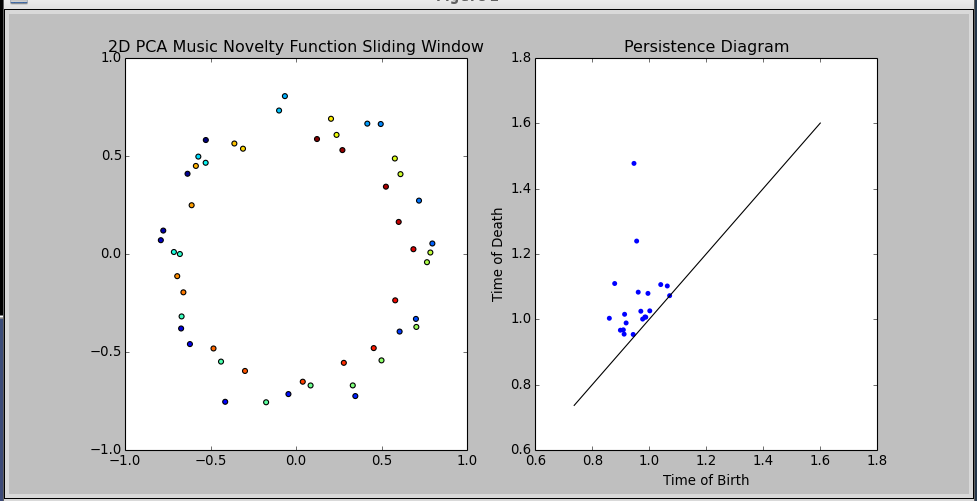
\includegraphics[width=0.8\textwidth]{pd.png}
\caption{1D Homology Persistence Diagram of MFCC Features from Voice Sample}
\end{figure}
\-\hspace{1cm} We then used the topological features and the raw audio
data as input to subsequent steps in the pipeline.

\subsection{Distance Metrics}
\-\hspace{1cm} We explored several different distance heurstics and metrics for
statistical comparisons and classification. Take note of their inputs, that is,
they are metrics and heuristics between different types of features, e.g.,
integer valued vectors, real valued vectors, signal functions, and persistence
diagrams.
\begin{enumerate}
  \item Real Valued Vector Spaces Euclidean Metric \newline $d : \mathbb{R}^n
  \times \mathbb{R}^n \rightarrow \mathbb{R}$ via $d(u,v) = \sqrt{\sum_{i=1}^{n}(u_i - v_i)^2}$
  \item Integer Valued Vector Spaces Canberra Metric \newline $d : \mathbb{Z}^n
  \times \mathbb{Z}^n \rightarrow \mathbb{R}$ via $d(u,v) = \sum_{i = 1}^{n} \frac{|x_i -
  y_i|}{|x_i| + |y_i|}$
  \item Integer Valued Vectors Spaces Bray-Curtis Metric \newline $d :
  \mathbb{Z}^n \times \mathbb{Z}^n \rightarrow \mathbb{R}$ via $d(u,v) = \frac{\sum_{i = 1}^{n}|x_i
  - y_i|}{\sum_{i = 1}^{n}|x_i + y_i|}$
  \item Real Valued Signal Inverse Max Cross Correlation \newline $d :
  \mathbb{C}^1 \times \mathbb{C}^1 \rightarrow \mathbb{R}$ via $d(f,g) =
  \frac{1}{\max _{\tau \in (-\infty,+\infty)} (\int _{-\infty}^{+\infty}
  f^{*}(t)g(t+\tau))}$
  \item Persistence Diagram Distance Multiscale Kernel \newline $d : PD \times
  PD \rightarrow \mathbb{R}$ via $d(P,Q) = \frac{1}{8 \pi \sigma} \sum_{p \in
  P, q \in Q}(\exp(-\frac{||p-q||^2}{8 \sigma}) -
  \exp(-\frac{||p-\bar{q}||^2}{8 \sigma}))$ where $||v||$ is the Euclidean
  Metric and if $q = (a,b)$, then $\bar{q} = (b,a)$. 
\end{enumerate}

\subsection{Statistics and Machine Learning}
\-\hspace{1cm} In our research, we wish to experiment with both the predictive
capablities of the distance functions with a variety of features. To
discriminate between voice samples from different people, we put the features
extracted from the samples into statistical tests and  classifiers with a
correspondingly appropriate distance metrics.
\subsubsection{Two Sample T Test}
\-\hspace{1cm} We took sets of feature vectors from voice samples of different
people, calculated distances between pairs of vectors within and pairs of
vectors across sets, and ran a two-sided t-test to determine whether the
distances of vector pairs within a set were statistically distinguishable from
the distances of vector pairs across sets. 
\newline \-\hspace{1cm} More concretely: first choose a feature and a
corresponding distance metric $d$. Let $C_i$ be collection of that feature
for person $i$. So, for instance, if the feature you chose was MFCC binned
persistence diagrams, then $C_i$ would be the set of MFCC binned persistence
diagrams for person $i$. Let $C_j, C_k$ feature from voice samples from 2
different people (i.e., 2 different classes).
For $C_k$ and $C_j$, construct $S_1$ and $S_2$ as follows: $S_1 =
\{d(x,y) : x, y \in C_k, x \neq y\}$ and $S_2 = \{d(x,y): x \in C_k, y \in
C_j\}$. Using $S_1$ and $S_2$, run a two sample t-test. The results of this test
will show whether the feature and distance metric chosen have discriminatory
power.
\subsubsection{Classifiers}
\-\hspace{1cm} We trained classifiers on feature vectors extracted from voice
samples of people and used the different distance metrics mentioned above for
classification. We experimented with both binary classification (using 2 labels
at a time) as well as multi-label (4 labels) classification. We use the
following sets of (feature, distance metric) pairs:
\begin{enumerate}
  \item (Binned Persistence Diagrams, Canberra Metric)
  \item (Binned Persistence Diagrams, Bray-Curtis Metric)
  \item (Binned Persistence Diagrams, Euclidean Metric)
  \item (Top 10 Persistence Bars, Euclidean Metric)
  \item (Raw Data, Inverse Cross Correlation)
  \item (Persistence Diagram, Multiscale Kernel Metric)
\end{enumerate}

\section{Results}
\subsection{Two Sample T Test Results}
\-\hspace{1cm} The results for a 2 sample T test are shown below for 2 of the
classes.
\begin{figure}[!ht]
\begin{center}
\begin{tabular}{||c|c|c||}
\hline
(feature, metric) & Test Statistics & P-Value \\ 
\hline 
Binned Persistence Diagrams, Canberra Metric & -21.420 & 9.848e-91 \\ 
\hline
Binned Persistence Diagrams, Bray-Curtis Metric & -7.481 & 1.185e-13 \\
\hline 
Binned Persistence Diagrams, Euclidean Metric & -4.218 & 2.601e-05 \\ 
\hline
Top 10 Persistence Bars, Euclidean Metric & 2.112 & 0.0348 \\
\hline
Raw Data, Inverse Cross Correlation & -0.337 & 0.736 \\
\hline
Persistence Diagram, Multiscale Kernel Metric & -2.405 & 0.016 \\
\hline
\end{tabular}
\end{center}
\caption{Binary Classification Average Results}
\end{figure}

\newpage
\subsection{Classification Results}
\-\hspace{1cm} The results for binary classification are shown below. Here, we
take all pairwise combinations of the classes and compute the percent of
correct true positives achieved by the (feature, metric) pair per combination.
The table shows the average of this percent across all combinations.
\begin{figure}[!ht]
\begin{center}
\begin{tabular}{||c|c|c||}
\hline
(feature, metric) & SVM & KNN \\ 
\hline 
Binned Persistence Diagrams, Canberra Metric & 0.140625 & 0.8125 \\ 
\hline
Binned Persistence Diagrams, Bray-Curtis Metric & 0.21875 & 0.78125 \\
\hline 
Binned Persistence Diagrams, Euclidean Metric & 0.36458333 & 0.77604167 \\ 
\hline
Top 10 Persistence Bars, Euclidean Metric & 0.48958333 & 0.53645833 \\
\hline
Raw Data, Inverse Cross Correlation & 0.42708333 & 0.71875 \\
\hline
Persistence Diagram, Multiscale Kernel Metric & 0.57291667 & 0.5 \\
\hline
\end{tabular}
\end{center}
\caption{Binary Classification Average Results}
\end{figure}

\begin{figure}[!ht]
\begin{center}
\begin{tabular}{||c|c|c||}
\hline
(feature, metric) & SVM & KNN \\ 
\hline 
Binned Persistence Diagrams, Canberra Metric & 0.0 & 0.5625 \\ 
\hline
Binned Persistence Diagrams, Bray-Curtis Metric & 0.046875 & 0.546875 \\
\hline 
Binned Persistence Diagrams, Euclidean Metric & 0.078125 & 0.515625 \\ 
\hline
Top 10 Persistence Bars, Euclidean Metric & 0.265625 & 0.15625 \\
\hline
Raw Data, Inverse Cross Correlation & 0.296875 & 0.59375 \\
\hline
Persistence Diagram, Multiscale Kernel Metric & 0.3125 & 0.25 \\
\hline
\end{tabular}
\end{center}
\caption{4 Multi-Label Classification Results}
\end{figure}
	
\section{Conclusion}
asdfs

\end{document}